% chapters/osfs.tex
%  Third chapter in osfs.tex

\section{Mathematical formulation of the Model}
One of the first attempts to solve this classical inverse problem was by Berthold K.P Horn by finding solutions of nonlinear first order partial differential equation called the \emph{brightness equation} under specific assumptions. This \emph{brightness equation} in simple words can be described as the map between the image intensities to the slope of the unknown surface, so that the shape can be constructed from the shading.\\

\noindent From Figure (\ref{fig:5}), in an orthographic camera model the surface point is directly projected onto the retinal plane in contrast to the perspective model which will be discussed in detail in Chapter $4$.\\

  \begin{figure}[h!]
  	\centering
  	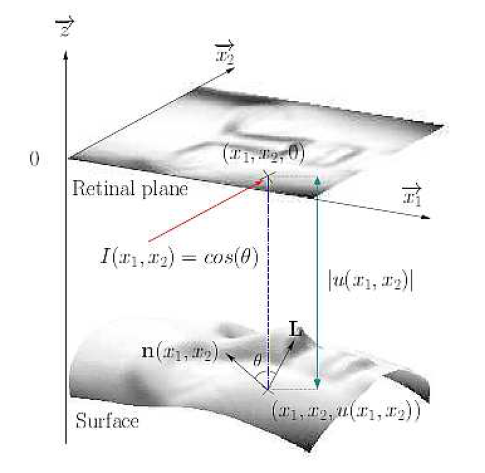
\includegraphics[scale = 0.3]{Images/orthographic_model.png}
  	\caption{Orthographic camera model}
  	\label{fig:5}
  \end{figure}
\pagebreak

\noindent The modelling of the problem leads to a partial differential equation. This equation arises from the following
\begin{equation}
I(x_1,x_2) = R(n(x_1,x_2))
\end{equation}	
where $(x_1,x_2)$ are the coordinates of a point $x$ in the image. The brighness equation is the relation between the reflectance map ($R$) to the brightness intensity ($I$). Almost all the shape from shading methods assume that the surface is \emph{Lambertian}. In this case, the reflectance map is the cosine of the angle between the light vector $\textbf{L}(x)$ and the normal vector $\textbf{n}(x)$ to the surface.
\begin{equation}
R = \cos(\textbf{L,n}) = \frac{\textbf{L}}{\lvert\textbf{L}\rvert}\cdot \frac{\textbf{n}}{\lvert\textbf{n}\rvert}
\end{equation}

\noindent Let $\Omega$ be an open subset of $ \mathbb{R}^2$ representing the image domain. For example $]a,b[ \times ]c,d[$.
\noindent In the Orthographic model we assume the light vector to be constant. We assume the light source to be unique and punctual. For $y \in \mathbb{R}^3$ , we denote $\mathbf{L}(y)$ the unit vector representing the light source direction at the point $y$. If the light source is located at infinity then the light vector field is uniform (i.e. constant). In this case, we denote by $\textbf{L} = (\alpha, \beta, \gamma)$ with $\gamma > 0$ and $\textbf{l} = (\alpha ,\beta)$. \\

\noindent Let us denote by $u$ the distance of the points in the scene to the camera. Now we have $\mathbf{n}(x) = (-\nabla u, 1)$. The SFS problem is then, given $I$ and \textbf{L}, to find a function $ u : \bar{\Omega} \rightarrow \mathbb{R}$ satisfying the brightness equation
\begin{equation}
	\forall x \in \Omega,  I(x) = \frac{-\nabla u(x) \cdot \mathbf{l} + \gamma}{\sqrt{1 + \lvert \nabla u(x) \rvert ^2}}
\end{equation}

\noindent This equation is rewritten, where $ p = \nabla u $. 
\begin{equation}
	H(x,p) = I(x)\sqrt{1+\lvert p \rvert^2} + p\cdot 1 - \gamma
\end{equation}
\noindent In our case we have considered a case where \textbf{L} = $(0,0,1)$ to obtain a Eikonal type equation where the function $H$ is called the \emph{Hamiltonian}.
\begin{equation}
	H_{Eiko} (x,p) = \lvert p \rvert - \sqrt{\frac{1}{I(x)^2} - 1}
\end{equation}

\section{Problem of Uniqueness}
\noindent Now consider the Eikonal equation in 1D,
\begin{eqnarray}
	\lvert u'(x)\rvert = 1 \qquad x\in (-1,1)\\
	u = 0 \qquad x\in \{-1,1 \}
\end{eqnarray}
\noindent The Hamiltonian $H(x,p) = \lvert p\rvert -1$ where $p=\nabla u$, is a covex function in $p$. We now show that the solution $u^+(x) = 1 - \lvert x\rvert$ is the viscosity solution to the problem.

\noindent \textbf{Proof:} Let $u-\phi$ attain maximum at $x_0$. In this case $x_0 = 0$.
\noindent This means,
\begin{eqnarray}
	u(x_0) - \phi(x_0) &\ge& u(x) - \phi(x) \qquad \forall x\in (-1,1) \\
	\implies \phi(x) - \phi(x_0) &\ge& u(x) - u(x_0)
\end{eqnarray}
\noindent If $x>x_0 =0$
\begin{eqnarray}
	\frac{\phi(x) - \phi(x_0)}{x-x_0} &\ge& \frac{u(x)-u(x_0)}{x-x_0} \\
	\implies \lim_{x\to x_0} \frac{\phi(x) - \phi(x_0)}{x-x_0}& \ge& \lim_{x\to x_0}\frac{u(x)-u(x_0)}{x-x_0}\\
	\phi' (x) &\ge& -1
\end{eqnarray}
\noindent If $x<x_0$, we follow the same procedure to get,
\begin{equation}
	\phi'(x) \le 1
\end{equation}
\noindent We get $\lvert \phi'(x)\rvert \le 1$, which shows that $u^+$ is a sub-solution to the Eikonal equation. One can verify that $u^+$ satisfies the super-solution condition as well and thus is a viscosity solution to the problem, which completes the proof.

\noindent It is easy to see that, by using the same steps, that $u^-(x) = \lvert x\rvert -1$ is \textbf{not a viscosity solution} if we choose the Hamiltonian $ H(x,p) = \lvert p\rvert -1$, but is indeed a viscosity solution for the Hamiltonian $H(x,p) = 1 - \lvert p \rvert$. Thus the viscosity solution is dependent on the nature of the Hamiltonian we choose, i.e., (concave or convex).

\noindent Let us consider the special case where the Eikonal equation is,
\begin{equation}
	\lvert \nabla u\rvert = 0
\end{equation}
\noindent This particular PDE presents us with a huge problem of \textbf{uniqueness}. This is evident from the sub-solution definition, that
\begin{eqnarray}
	H(x.\nabla\phi) \le 0 \\
	\implies \lvert \nabla\phi\rvert \le 0
\end{eqnarray}
\noindent which cannot be satisfied for all cases, as $\lvert\nabla\phi\rvert \ge 0$. This particular case is a problem when we consider the numerical solution of the Shape from Shading Model proposed by Rouy and Tourin \cite{rouy}.

\noindent Subsolution condition is satisfied as long as $0 < I(x) < 1$, and the uniqueness is lost as soon as $I(x) = 1$. These places where $I(x) = 1$ are called the \textbf{singularity points} where \emph{the solution has to specified in order to obtain the relevent solution}.